\section{Bazar Blot Game}\label{ModelDescription}
\lhead{AI algorithms used for the game}
\subsection{Hill Climbing Algorithm for Bidding}
\hspace{\parindent}You can find a provided template for the Belote AI model.
The general environment consists of a player and 3 AIs; let’s call them \textit{Left
AI}, \textit{Right AI} and \textit{Top AI}. The first stage of the game is the implementation of
the bidding part, where each player should bid a number for the hand they received
and try to negotiate with their partner. We decided to use the Hill-Climbing Algorithm by
using a manual and mildly complicated heuristic for each player pair and each
possible suit available to bid on (\textit{Spades, Hearts, Diamonds, Clubs, No-Trumps}). The
Algorithm will count the heuristic value for each suit, compare it to the opponents’
bid, and take into account the partner’s previous bid. The main operation will include
giving a weight to the higher cost cards (Aces and Tens for the Suit “Aces”, Jacks and
Nines for the rest), add the partner’s bid to the corresponding suit, find the maximum
among the 5 possibilities, and compare it to the opponents’ bid.
\par Scenario


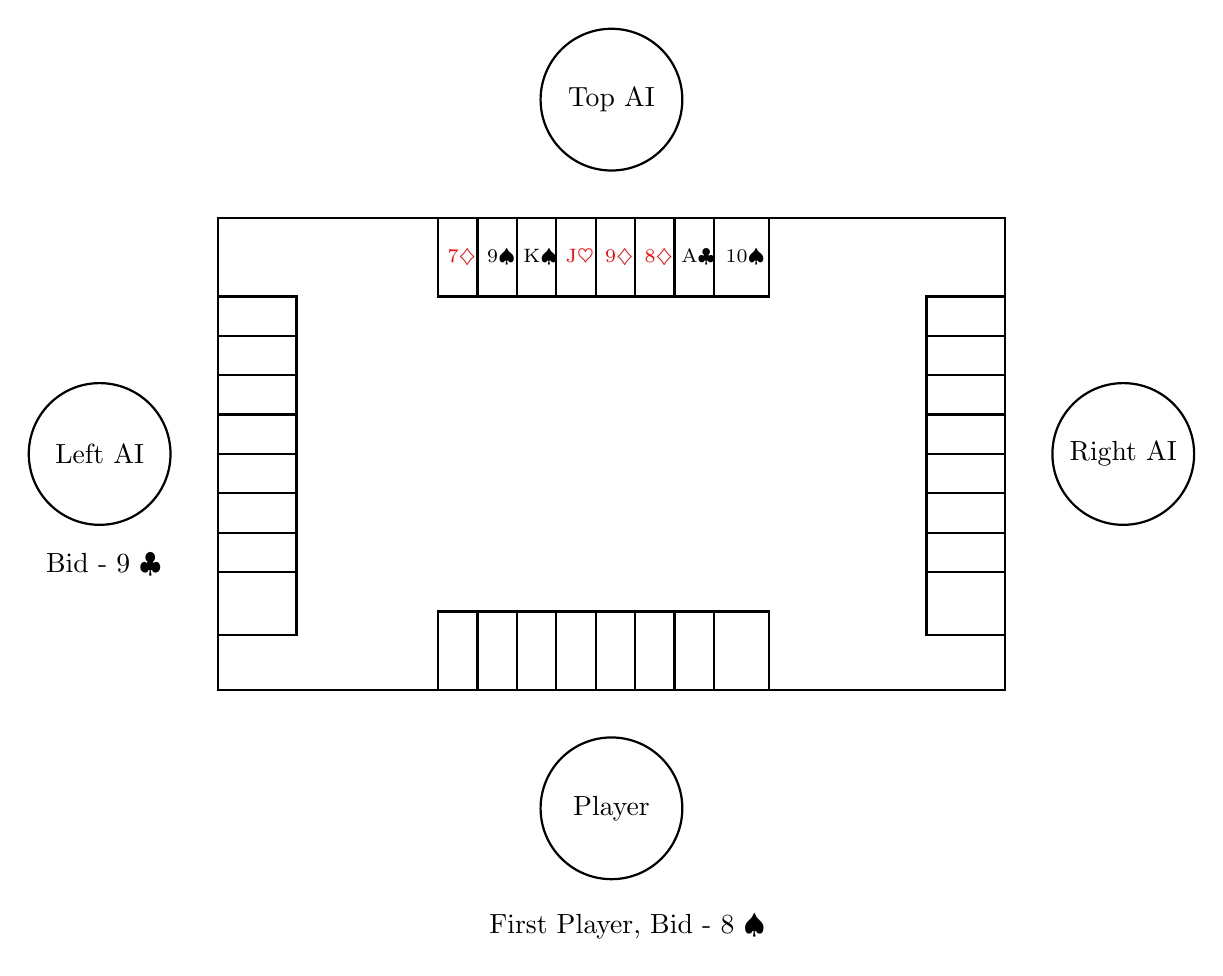
\begin{tikzpicture}

\draw[thick] (0,0) rectangle (10,6);  % Rectangle table dimensions

\foreach \i in {0,1,2,3,4,5,6,7}
    \draw[thick, draw=black, fill=white] (1, 5-\i*0.5) rectangle (0, 5-\i*0.5-0.8);
\foreach \i in {0,1,2,3,4,5,6,7}
    \draw[thick, draw=black, fill=white] (10, 5-\i*0.5) rectangle (9, 5-\i*0.5-0.8);
\foreach \i in {0,1,2,3,4,5,6,7}
    \draw[thick, draw=black, fill=white] (2.8 + \i*0.5, 6) rectangle (3.5 + \i*0.5, 5);
\foreach \i in {0,1,2,3,4,5,6,7}
    \draw[thick, draw=black, fill=white] (2.8 + \i*0.5, 0) rectangle (3.5 + \i*0.5, 1);

\draw[thick] (-1.5, 3) circle(0.9);
% Right side chair
\draw[thick] (11.5, 3) circle(0.9);
% Top side chair
\draw[thick] (5, 7.5) circle(0.9);
% Bottom side chair
\draw[thick] (5, -1.5) circle(0.9);

\node at (-1.5, 3) {Left AI};
\node at (-1.45, 1.6) {Bid - 9 $\clubsuit$};
\node at (11.5, 3) {Right AI};
\node at (5, 7.5) {Top AI};
\node at (5, -1.5) {Player};
\node at (5.2, -3) {First Player, Bid - 8 $\spadesuit$};

\node at (3.1, 5.5) {\scriptsize \textcolor{red}{7$\diamondsuit$}};
\node at (3.6, 5.5) {\scriptsize \textcolor{black}{9$\spadesuit$}};
\node at (4.1, 5.5) {\scriptsize \textcolor{black}{K$\spadesuit$}};
\node at (4.6, 5.5) {\scriptsize \textcolor{red}{J$\heartsuit$}};
\node at (5.1, 5.5) {\scriptsize \textcolor{red}{9$\diamondsuit$}};
\node at (5.6, 5.5) {\scriptsize \textcolor{red}{8$\diamondsuit$}};
\node at (6.1, 5.5) {\scriptsize \textcolor{black}{A$\clubsuit$}};
\node at (6.7, 5.5) {\scriptsize \textcolor{black}{10$\spadesuit$}};

\end{tikzpicture} \pagebreak

If at the start of the game you recalled 8 Spades, and the opponent (Left AI), raised the bid to 9 Clubs,
your partner’s algorithm will look into the hand; say it has these cards (7$\diamondsuit$, 9$\spadesuit$, King$\spadesuit$,
Jack$\heartsuit$, 9$\diamondsuit$, 8$\diamondsuit$, Ace$\clubsuit$, 10$\spadesuit$). The heuristic value for each of the suits would be;

\begin{itemize}
    \item Diamonds:  14 = 0 (8$\diamondsuit$) + 14 (9$\diamondsuit$) + 0 (7$\diamondsuit$),
    \item Spades: 32 = 4 (King$\spadesuit$) + 14 (9$\spadesuit$) + 10 (1$\spadesuit$0) + 1/2 x 8 (Partner’s Bid),
    \item Hearts: 20 (Jack $\heartsuit$),
    \item Clubs: 6.5 = 11 (Ace$\clubsuit$) - 1/2 x 9  (Opponents’ Bid),
    \item No Trumps: 25 = 4 (King$\spadesuit$) + 19 (Ace$\clubsuit$) + 2 (Jack$\heartsuit$)
\end{itemize}

Here it is obvious that the AI
is going to call its partner’s bid (Spades, as it has the highest heuristic value), the question is: How much? There is another logic
imported that would decide if there is a need for the AI to increase the bid by 1, 2 or
more, and the main logic is going to contain the possible additional points from special
combinations (like Tierce giving 2 points), it will also include the bade suit heuristic
value divided 20 (as each 10 heuristic equals to 1 point, and divided with another 2 for emergency)
and rounded and will be added to the point
count, in this case we will have a Tierce (7$\diamondsuit$, 8$\diamondsuit$, 9$\diamondsuit$) and heuristic difference of 32/20
= 1.6, rounded to 2. The point count would include adding 4 points to the partner’s bid,
hence the algorithm will return 12 Spades. There are going to be extra conditions for
the actions Coinchee, Cabot, etc.)


\subsection{Minimax Algorithm for the Playing part}
\hspace{\parindent} In the second part of the game one of the available options is stochastic Minimax.
This algorithm consists of Min, Max and Chance nodes, the problem lies in the chance nodes which have a lot of nodes coming out of them.
For example consider the first hand in the game when the bot has to make a move. Lets say the bot is a max node.
The bot can make 8 moves so there are 8 branches coming out of the root. Next we need to have chance nodes coming out of each of the 8 nodes.
The chance nodes each have $\binom{24}{8}$ nodes since that's how many possible combination of cards the next player can have.
This by itself already renders the Minimax algorithm not practical since it is not feasible to check that many nodes.
For example consider the case when \textbf{DESCRIBE THE TEXT HERE}: \\
\textbf{ADD GRAPHIC HERE}